\begin{tikzpicture}[x=1pt,y=1pt,
    every node/.style={font=\small},
    ah/.style={draw opacity=0,line width=0.08,fill opacity=1},
    lbl/.style={fill=white,fill opacity=0.88,text opacity=1,
                align=center,inner sep=2.5pt,line width=0.6pt},
    wire/.style={line width=0.75pt},
    inst/.style={align=center,inner sep=1pt},
    panel/.style={font=\normalsize\bfseries,anchor=north,inner sep=0pt}]

% =======================================================================
% (a) Radiograph, 200 x 173.7
% =======================================================================
\node [anchor=south west,inner sep=0] at (0,0)
  {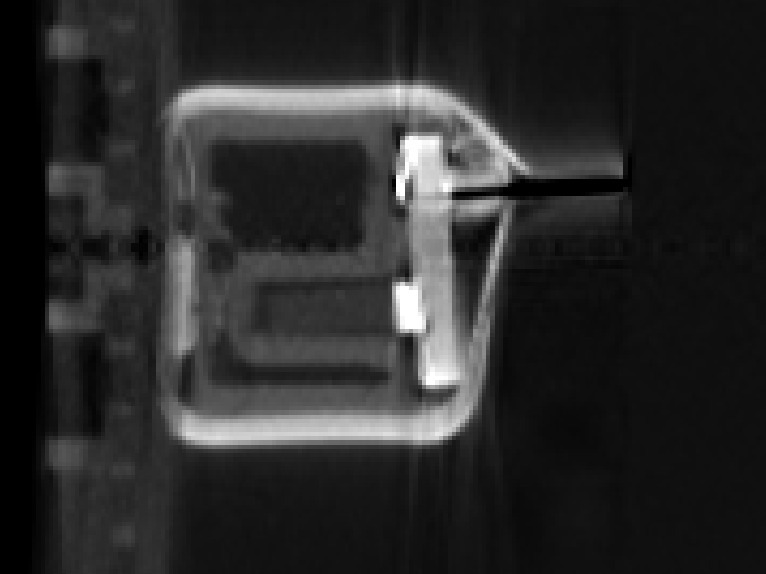
\includegraphics[width=200pt,height=173.7pt,interpolate=true]{images/sipm_fibre.jpg}};

% ---- 3D-printed enclosure ----------------------------------------------
\node [lbl,draw={rgb, 255:red, 81; green, 81; blue, 81 },anchor=north west]
      (enc) at (4,169.7) {3D-printed\\Enclosure};
\draw [color={rgb, 255:red, 81; green, 81; blue, 81 },line width=1.1pt]
      (enc.south) |- (51.4,135.1);
\draw [shift={(59.3,135.1)},rotate=180,ah,fill={rgb, 255:red, 81; green, 81; blue, 81 }]
      (7.85,-3.78) -- (0,0) -- (7.85,3.78) -- cycle ;

% ---- Pin header --------------------------------------------------------
\node [lbl,draw={rgb, 255:red, 204; green, 153; blue, 0 },anchor=north east]
      (pin) at (196,169.7) {Pin Header};
\draw [color={rgb, 255:red, 204; green, 153; blue, 0 },line width=1.1pt]
      (pin.south) |- (160.2,118.5);
\draw [shift={(152.3,118.5)},rotate=0,ah,fill={rgb, 255:red, 204; green, 153; blue, 0 }]
      (7.85,-3.78) -- (0,0) -- (7.85,3.78) -- cycle ;

% ---- PCB ---------------------------------------------------------------
\node [lbl,draw={rgb, 255:red, 55; green, 173; blue, 107 },anchor=east]
      (pcb) at (196,94.5) {PCB};
\draw [color={rgb, 255:red, 55; green, 173; blue, 107 },line width=1.1pt]
      (pcb.west) -- (119.3,94.5);
\draw [shift={(111.4,94.5)},rotate=0,ah,fill={rgb, 255:red, 55; green, 173; blue, 107 }]
      (7.85,-3.78) -- (0,0) -- (7.85,3.78) -- cycle ;

% ---- SiPM --------------------------------------------------------------
\node [lbl,draw={rgb, 255:red, 26; green, 111; blue, 223 },anchor=east]
      (sipm) at (196,50) {SiPM};
\draw [color={rgb, 255:red, 26; green, 111; blue, 223 },line width=1.1pt]
      (sipm.west) -| (106.8,70.7);
\draw [shift={(106.8,78.6)},rotate=-90,ah,fill={rgb, 255:red, 26; green, 111; blue, 223 }]
      (7.85,-3.78) -- (0,0) -- (7.85,3.78) -- cycle ;

% ---- Fibre -------------------------------------------------------------
\node [lbl,draw={rgb, 255:red, 241; green, 74; blue, 64 },anchor=west]
      (fib) at (4,50) {Fibre};
\draw [color={rgb, 255:red, 241; green, 74; blue, 64 },line width=1.1pt]
      (fib.east) -| (82.6,73.7);
\draw [shift={(82.6,81.6)},rotate=-90,ah,fill={rgb, 255:red, 241; green, 74; blue, 64 }]
      (7.85,-3.78) -- (0,0) -- (7.85,3.78) -- cycle ;

\node [panel] at (100,-8) {(a)};

% =======================================================================
% (b) Circuit, loop 160 x 139, centred in a 200 x 173.7 slot (x = 230 to 430)
% =======================================================================
\path (230,0) rectangle (430,173.7);

\draw [wire] (250,98.1) -- (250,156.35) -- (323,156.35);
\draw [wire] (337,156.35) -- (410,156.35) -- (410,101.85);
\draw [wire] (410,71.85) -- (410,17.35) -- (250,17.35) -- (250,75.6);

% ---- 6487 voltage source -----------------------------------------------
\draw [wire] (239,98.1) -- (261,98.1);
\draw [wire] (244,90.6) -- (256,90.6);
\draw [wire] (239,83.1) -- (261,83.1);
\draw [wire] (244,75.6) -- (256,75.6);
\node at (237,108) {$+$};
\node at (237,65.7) {$-$};
\node [anchor=west] at (252,109) {HI};
\node [anchor=west] at (252,64.7) {LO};
\node [inst,anchor=west] at (268,86.85) {6487\\$V_{bias}$};

% ---- SiPM --------------------------------------------------------------
\draw [wire,fill=white] (337,163.85) -- (323,156.35) -- (337,148.85) -- cycle;
\draw [wire] (323,163.85) -- (323,148.85);
\node [anchor=north,inner sep=2pt] at (330,146.5) {SiPM};

% ---- 6487 picoammeter --------------------------------------------------
\draw [wire,fill=white] (410,86.85) circle [radius=15];
\node at (410,86.85) {\textbf{A}};
\node [anchor=east] at (408,111) {HI};
\node [anchor=east] at (408,62.7) {LO};
\node [inst,anchor=east] at (389,86.85) {6487\\Picoammeter};

\node [panel] at (330,-8) {(b)};

\end{tikzpicture}%